\documentclass{book}

\usepackage{amsmath}
\usepackage{amssymb}
\usepackage{chemfig}
\usepackage{mathtools}
\usepackage{listings}
\usepackage{wrapfig}
\usepackage{color}
\usepackage{float}
\usepackage{caption}
\usepackage{subcaption}
\usepackage{multicol}
\usepackage{paralist}
\usepackage{tcolorbox}
\usepackage{braket}
\usepackage[framemethod=TikZ]{mdframed}
\usepackage[english]{babel}
\usepackage[utf8x]{inputenc}
\usepackage[colorinlistoftodos]{todonotes}
\usepackage{esint}
\usepackage{hyperref}

\title{Algorithmic Theory}
\date{2019-01-01}
\author{Animesh Sinha; Gaurang Tandon; Arpan Dasgupta; }

\lstdefinestyle{shared}{
    belowcaptionskip=1\baselineskip,
    breaklines=true,
    xleftmargin=\parindent,
    showstringspaces=false,
    basicstyle=\fontsize{10}{6}\ttfamily,
}
\lstdefinestyle{cpp}{
	style=shared,
    language=C++,
    keywordstyle=\bfseries\color{green!40!black},
    commentstyle=\itshape\color{red!80!black},
    identifierstyle=\color{blue},
    stringstyle=\color{purple!40!black},
}
\lstdefinestyle{java}{
    style=shared,
    language=Java,
    keywordstyle=\bfseries\color{green!40!black},
    commentstyle=\itshape\color{purple!40!black},
    identifierstyle=\color{blue},
    stringstyle=\color{orange},
}
\lstdefinestyle{py}{
    style=shared,
    language=Python,
    keywordstyle=\bfseries\color{green!40!black},
    commentstyle=\itshape\color{purple!40!black},
    identifierstyle=\color{blue},
    stringstyle=\color{orange},
}
\lstdefinestyle{txt}{
    style=shared,
}
\lstset{escapechar=@}

\newcounter{theo}[section]\setcounter{theo}{0}
\renewcommand{\thetheo}{\arabic{section}.\arabic{theo}}
\newenvironment{theorem}[2][]{%
\refstepcounter{theo}%
\ifstrempty{#1}%
{\mdfsetup{%
frametitle={%
\tikz[baseline=(current bounding box.east),outer sep=0pt]
\node[anchor=east,rectangle,fill=blue!20]
{\strut Theorem~\thetheo};}}
}%
{\mdfsetup{%
frametitle={%
\tikz[baseline=(current bounding box.east),outer sep=0pt]
\node[anchor=east,rectangle,fill=blue!20]
{\strut Theorem~\thetheo:~#1};}}%
}%
\mdfsetup{innertopmargin=10pt,linecolor=blue!20,%
linewidth=2pt,topline=true,%
frametitleaboveskip=\dimexpr-\ht\strutbox\relax
}
\begin{mdframed}[]\relax%
\label{#2}}{\end{mdframed}}


\newcounter{prf}[section]\setcounter{prf}{0}
\renewcommand{\theprf}{\arabic{section}.\arabic{prf}}
\newenvironment{proof}[2][]{%
\refstepcounter{prf}%
\ifstrempty{#1}%
{\mdfsetup{%
frametitle={%
\tikz[baseline=(current bounding box.east),outer sep=0pt]
\node[anchor=east,rectangle,fill=red!20]
{\strut Proof~\theprf};}}
}%
{\mdfsetup{%
frametitle={%
\tikz[baseline=(current bounding box.east),outer sep=0pt]
\node[anchor=east,rectangle,fill=red!20]
{\strut Proof~\thetheo:~#1};}}%
}%
\mdfsetup{innertopmargin=10pt,linecolor=red!20,%
linewidth=2pt,topline=true,%
frametitleaboveskip=\dimexpr-\ht\strutbox\relax
}
\begin{mdframed}[]\relax%
\label{#2}}{\end{mdframed}}


\newcounter{exm}[section]\setcounter{exm}{0}
\renewcommand{\theexm}{\arabic{section}.\arabic{exm}}
\newenvironment{example}[2][]{%
\refstepcounter{exm}%
\ifstrempty{#1}%
{\mdfsetup{%
frametitle={%
\tikz[baseline=(current bounding box.east),outer sep=0pt]
\node[anchor=east,rectangle,fill=green!20]
{\strut Example~\theexm};}}
}%
{\mdfsetup{%
frametitle={%
\tikz[baseline=(current bounding box.east),outer sep=0pt]
\node[anchor=east,rectangle,fill=green!20]
{\strut Example~\thetheo:~#1};}}%
}%
\mdfsetup{innertopmargin=10pt,linecolor=green!20,%
linewidth=2pt,topline=true,%
frametitleaboveskip=\dimexpr-\ht\strutbox\relax
}
\begin{mdframed}[]\relax%
\label{#2}}{\end{mdframed}}


\newcounter{def}[section]\setcounter{def}{0}
\renewcommand{\thedef}{\arabic{section}.\arabic{def}}
\newenvironment{definition}[2][]{%
\refstepcounter{def}%
\ifstrempty{#1}%
{\mdfsetup{%
frametitle={%
\tikz[baseline=(current bounding box.east),outer sep=0pt]
\node[anchor=east,rectangle,fill=yellow!20]
{\strut Definition~\thedef};}}
}%
{\mdfsetup{%
frametitle={%
\tikz[baseline=(current bounding box.east),outer sep=0pt]
\node[anchor=east,rectangle,fill=yellow!20]
{\strut Definition~\thetheo:~#1};}}%
}%
\mdfsetup{innertopmargin=10pt,linecolor=yellow!20,%
linewidth=2pt,topline=true,%
frametitleaboveskip=\dimexpr-\ht\strutbox\relax
}
\begin{mdframed}[]\relax%
\label{#2}}{\end{mdframed}}

\let\cleardoublepage\clearpage


\begin{document}
\pagenumbering{arabic}


\begin{titlepage}
    \newcommand{\HRule}{\rule{\linewidth}{0.5mm}}
    \center
    \textsc{\LARGE International Institute of Information Technology, Hyderabad}\\[0.5cm]
    
\includegraphics[scale=1]{img/iiit-logo.jpeg}\\[0.5cm]
    \textsc{\Large Algorithmic Theory}\\[0.5cm]
    \textsc{\large Data Structures, Algorithms and Competitive Programming}\\[0.5cm] % Minor heading such as course title
    \HRule \\[0.4cm]
    { \huge \bfseries College Notes}\\[0.4cm]
    \HRule \\[1.5cm]
    \begin{minipage}{0.6\textwidth}
    \begin{flushleft} \large
    \emph{Maintainers:} Animesh Sinha, Gourang Tandon, Arpan Dasgupta, Yogottam Khandelwal, Aman Kumar Singh.
    \end{flushleft}
    \end{minipage}\\[2cm]
    {\large \today}\\[2cm]
    \vfill
\end{titlepage}

\chapter{Heaps}



\section{Question Patterns}


\subsection{Generic Types}

\begin{itemize}
    \item Find the kth Minimum or Maximum. This can also be on arrays or trees with online insertion or deletion.
    \item Priority Queue questions. Typically greedy algorithms best implemented this way. (eg. Dijkstra)
\end{itemize}


\subsection{Specific Illustrations}

\paragraph{When not to use Heaps} \textit{Question: Find the kth-Maximum sum of all subarrays of any given array}. This question demostrates that when we have \textbf{k-sorted elements appended to our queue of k-maximum elements} at one go, it's better to use an actual \textbf{Sorted array and the Merge Function for Updates}.

\paragraph{Lazy Deletion} Heaps cannot search, so heaps cannot delete. A simple solution for this is to maintain another heap of all deleted elements, and if the actual heap and deleted heap have the same top element, keep popping them out. We only care about the top element, so we can be Lazy in the deletion of the elements lower down in the tree.



\section{Elementary Theory}


\subsection{Basic Operations}

\paragraph{Heapification}
A \textbf{O(n)} algorithm exists for Heapification. It uses the standard sift-down procedure, but starts by correcting the lowest layers first. So start at the end of the array and move back.

\paragraph{Insert}
A \textbf{O(log n)} algorithm is used to insert. We push the element at the end of the array and sift-up or sift-down the element till the element is at a valid locale. 

\paragraph{Delete}
For a \textbf{O(log n)} deletion algorithm, we must swap the last element with the element to be deleted, sift-up/down the former last element, and pop-out the last element.
This is only possible if we have a refernce to the element, search and delete take O(n) time to perform on heaps.

\paragraph{Minimum/Maximum}
Minimum on a MinHeap takes \textbf{O(1)} time, and so does Maximum on a MaxHeap.

\subsection{Implementation Code}

\lstinputlisting[basicstyle=Large,style=cpp]{code/BinaryHeap.hpp}
\chapter{Range Queries}



\section{Square Root Decomposition}

Break the array down into chunks of $\sqrt{n}$. Store the answer to these chunks. The answer to range queries is the answer in the starting chunk after L, plus in the ending chunk before R, plus the stored results of everything in between. Updates can be done in $O(\sqrt{n})$ steps by just updating the result of the chunk.

\subsection{Motivating Examples}

This cannot be solved by a Segment Tree (easily).

\begin{example}{q-rmq-01}
    \textbf{Question: Given and array, support update and query operation for number of elements less than k in the given range.} \\
    Solution: Maintain sorted vector of each block of the square-root decomposition. Search over all blocks and find lowerbound(k), the sum of these counts gives the answer in $O(\sqrt{n} log(n))$. For update, just sort again, using insertion sort you get $O(\sqrt{n})$.
\end{example}



\section{Mo's Algorithm}

This is an algorithm to handle offline queries by sorting them and trying to cleverly avoid recomputing portions that were already solved \relax for in the previous queries.
(Direcly usable with associative, commutative, invertible operations).

\subsubsection{Algorithm}
Break down the array in blocks of size $\sqrt{n}$. Sort queries by starting block, them by ending position. The right pointer keeps moving forward for each block, the left pointer keeps moving back and forth withing a block, adding elements as it goes back and subtracting as it goes forth. This results in all queries being solved in $O(n\sqrt{n})$ time.

\begin{example}{q-rmq-02}
    \textbf{Question: Given an array, find the number of elements distinct elements in range (l, r).}
    Sort the queries first by the starting block, then by the end position. Maintian a frequency array of all elements currently between right and left pointers. For each of the $O(\sqrt{n})$ blocks, the start pointer moves atmost $O(\sqrt{n})$ times back and forth in the block, adding and deleting elements. For each block the right pointer only goes forward adding in elements, $O(\sqrt{n})$ blocks each taking $O(n)$ time.
\end{example}

\begin{example}{q-rmq-03}
    \textbf{Question: Given an array, find the f(s)*f(s)*s for all distinct s in range (l, r), where f(s) is the frequency of s.} \\
    Same Algorithm, and same frequency array as above, just find $f(s)*f(s)*s$ instead of $\delta(f(s))$ as above.
\end{example}

\chapter{Dynamic Programming}

The focus of this chapter would be to enlist all the optimizations to a DP possible and types of recurrences solvable using them.



\section{Matrix Exponentiation}


\begin{example}{}
\textbf{Number of ways to construct an array starting in X, and ending in Y, with no two adjacent elements are the same.}
\begin{equation*}
    dp[i] = \begin{bmatrix} dp[i][\text{CLASH}] \\ dp[i][\text{CLEAN}] \end{bmatrix}
    = \begin{bmatrix} 0 & 1 \\ k-1 & k-2 \end{bmatrix} \times dp[i-1]
\end{equation*}
\end{example}

\chapter{Game Theory}



\section{NIM Games and Sprague-Grundy Theorem}



\section{Take Away Games}


\subsection{Identifying the Losing States}

\begin{theorem}{Take Away}
  Let $H_i$ denote all the losing states, and $f(x)$ denote the number of stones that can be removed in the next move after x stones in the previous. Then we can find the losing states as follows.
  \begin{equation}
    H_{k+1} = H_k + H_m, \;\;\;\;\; where \;\; m = min \{j: f(H_j) \geq H_k\}
  \end{equation}
\end{theorem}
The idea is that we can remove any $H_j + H_k$ stones, we can think of them as two separate piles. We cannot win on either pile, so the only way to win is when the $H_j$ pile ends, the last move was enough that $f(last\:move) \geq H_k$ so that we can win next move. If this is not possible, then the state is losing.

\textbf{KEY IDEA: Find the RECURRENCE, make a SOLUTION HYPOTHESIS by monitoring the pattern and prove it BY INDUCTION to get all the losing states.}


\subsection{A few Example Functions}

\subsubsection{Example: f(x) = x}
1 stone is losing, so $H_1 = 1$. And whenever $H_k$ is losing, the $min\{H_j : f(H_j) \geq H_k\} = min\{H_j : H_j \geq H_k\} = H_k$, therefore the losing states are $2^n$.
\subsubsection{Example: f(x) = 2x - 1}
1 stone is losing, so $H_1 = 1$. Our Hypothesis, $H_k = 2 H_{k-1}$. And whenever $H_k$ is losing, the $min\{H_j : f(H_j) \geq H_k\} = min\{H_j : 2*H_j-1 \geq H_k\} = H_k$, therefore the losing states are $2^n$.
\subsubsection{Example: f(x) = 2x: Fibonacci NIM}
1 stone is losing, so $H_1 = 1$. Our Hypothesis, $H_k = H_{k-1} + H_{k-2}$. And whenever $H_k$ is losing, the $min\{H_j : f(H_j) \geq H_k\} = min\{H_j : 2*H_j \geq H_k\} = H_{k-1}$, therefore the losing states are the Fibonacci numbers.


\subsection{Winning Strategy}

\subsubsection{New Binary number systems}
We find that we can express any number as a sum of the values of $H_1$, $H_2$, ..., so we construct a binary like number system where a the place value of the i-th digit is $H_i$ and the face value is 0 or 1. Let's call this H-binary. (Note: This expression is unique and complete for powers of 2, and for the Fibonacci numbers - Zeckendorf theorem, as in the above examples).

\subsubsection{The greedy strategy}

Given any starting state that is not losing, we can write out it's representation in the H-Binary system.
Since this will have more than 1 ones in it's representation, \colorbox{yellow}{we subtract the LEAST SIGNIFICANT BIT}.

Now, the opponent cannot remove the next one in the representation, because of the property of number systems that $H_j > f(H_i) \;\; \forall j > i$, due to the way we found losing states $H_i$. Finally, when our oppnent removes any value from the form $.....1000000$ (Any value, last set bit 1, and 0s), he will get a 1 in the resulting representation $.....0000110$.

Now in our move we shall remove the lowest set bit again. This is possible, as the last move must have been greater than or equal to $H_j$ if j is lowest set bit. (Obviously, because when we add back we need to have 1+1 = 0 to get all the numbers back to 0 and 1 at the position that could not be removed). So $f(H_j) >= H_j$, this move is possible, and we can win.

\subsection{Proof of Victory}
On our moves, we reduce the number of ones in the representation by 1. Our opponent, if he removes the one at $H_j$, he has to insert a 1 and position smaller than j. So he increases or keeps constant the number of ones. Obviously, the last move will be played by us, reducing the number of ones to 0 and finishing the game.


\subsection{References}

\subsubsection{Problems}
Fibonacci Nim (Direct Implementation) [ICPC Kolkata 2018] \url{https://www.codechef.com/KOL18ROL/problems/SNOWMAN}

\subsubsection{Theory}
Contains most of the theory mentioned above: \url{http://www.cut-the-knot.org/Curriculum/Games/TakeAway.shtml#theory}



\section{Finding Invarients}

\textbf{Mark out a state and all it's children. Either try MINIMAX TREE, and if the state space is large, try to find invarients, specially MODULO or PARITY.}

\begin{example}[Invarients in Games - 1]{exm:invarients-stick-game-1}
  \textbf{Question: Start with \{(4 sticks, length 4), (1 stick, length 1)\}. In a move, we can break a stick or remove k sticks of length k. Last move wins. Find the winning states \& strategy.}
  Any state be (n1, n2, n3, n4). All states with (n1 + n3) \% 2 == (n2 + n4) \% 3 are winning positions, all others are losing. We can prove than any winning position goes to losing position and vice-versa.
\end{example}

\chapter{Mathematical Tools}


% Fast Fourier Transforms

\section{Fast Fourier Transforms}


\subsection{Motivation and Purpose}

We want to be able to interconvert a polynomial between \textbf{SAMPLES representation and COEFFICIENTS representation}.

\paragraph{} A n-degree polynomial can be a n-dimentional COEFFICIENTS vector where it is easy to compute the value at any random x, and as a n-dimentional SAMPLES vector that has n (x, y) pairs, making it easy to multiply vectors. If we can convert back and forth in $O(n \cdot log(n))$, and \textit{multiply polynomials} in SAMPLES land in $O(n)$, then we get a speed up over the typical $O(n^2)$ for multipling each coefficient with every other.


\subsection{Algorithm}

\subsubsection{The Recurrence}

Given a polynomial $P(x)$, to convert it into samples at $X = \{X_1, X_2 ..., X_n\}$.
We can solve it using the recurrence
\begin{equation}
  P(X) = P_{even}(x^2) + x \cdot P_{odd}(x^2)
\end{equation}
where $P_{even}$ is the polynomials with only even coefficients, $P_{odd}$ with only odd.
Note that the degree of the resulting polynomials $P_{even}$ and $P_{odd}$ is half of the original.

\subsubsection{The Complex Numbers}

We also want the size of the set X, at which we have to evaluate the polynomial to go down. So we can use complex numbers, for polynomial of degree n, we use \textbf{the $2^k$-roots of unity} where $2^k$ is the smallest value power of 2 bigger than n.

The set will keep collapsing to half it's size after each step, as squares of exactly two of these roots is the same.

\subsubsection{The Divide and Conquer}
In summary, we are performing a Divide and Conquer solve, where each state is <P, X>.
We start with our \textbf{Original P, and X = 1}. In each divide step, we split the P into two parts, and each part gets one root of X, here +1 and -1. Then that divides in 4, at values +i, -i, +1 and -1. There are log(n) layers with $2^l$ polynomials of size $n/2^l$, each polynomial is to be evaluated at 1 value.


\subsection{Some Mathematical Representations}

\begin{equation}
  \begin{bmatrix}
    1   & x_1^2 & x_1^3 & x_1^4 & ... & x_1^n \\
    1   & x_2^2 & x_2^3 & x_2^4 & ... & x_2^n \\
    1   & x_3^2 & x_3^3 & x_3^4 & ... & x_3^n \\
    ... & ...   & ...   & ...   & ... & ...   \\
    1   & x_n^2 & x_n^3 & x_n^4 & ... & x_n^n \\
  \end{bmatrix} \times
  \begin{bmatrix}
    c_1 \\ c_2 \\ c_3 \\ ... \\ c_n
  \end{bmatrix} =
  \begin{bmatrix}
    s_1 \\ s_2 \\ s_3 \\ ... \\ s_n
  \end{bmatrix}
\end{equation}

Here we have the Vandermond Matrix of a set of N values for X times the coefficient vector gives the samples vector. We decided to choose our values in X as such:
$ X = \{ 1, \omega_n, \omega_n^2, \omega_n^3, ..., \omega_n^{n-1} \} $.

\subsection{Inverse Fourier Transform}

\begin{equation}
  \begin{bmatrix}
    1   & 1              & 1               & 1               & ... & 1                     \\
    1   & \omega_n^1     & \omega_n^2      & \omega_n^3      & ... & \omega_n^{ n-1}       \\
    1   & \omega_n^2     & \omega_n^4      & \omega_n^6      & ... & \omega_n^{2n-2}       \\
    ... & ...            & ...             & ...             & ... & ...                   \\
    1   & \omega_n^{n-1} & \omega_n^{2n-2} & \omega_n^{3n-3} & ... & \omega_n^{(n-1)(n-1)} \\
  \end{bmatrix} ^{-1} \times
  \begin{bmatrix}
    s_1 \\ s_2 \\ s_3 \\ ... \\ s_n
  \end{bmatrix} =
  \begin{bmatrix}
    c_1 \\ c_2 \\ c_3 \\ ... \\ c_n
  \end{bmatrix}
\end{equation}
Here is the definition of the operation. We are going from samples to coefficient, so we need multiplication by inverse of the matrix for Fourier. This is easy, because the inverse is just the complex conjugate divided by n.
\begin{equation}
  V^{-1} = \bar{V} / n
\end{equation}

So we can use the FFT Algorithm again, since $X = {1, \bar{\omega}^1, \bar{\omega}^2, \bar{\omega}^3, ..., \bar{\omega}^n}$. And divide the answer by n. Note that X is still the same set, so no change to FFT is needed.


\subsection{Number Theoretic Transforms}

The number theoretic transform is based on generalizing the n-th primitive root of unity to a "quotient ring" instead of the usual field of complex numbers.

We take a number $w$ that satisfies $w^n \equiv 1 (mod p)$ going through each of the numbers only and atmost once.

% Group Theory

\section{Group Theory}


\subsection{Burnside's Lemma}

It states the number of elements in the Orbit of a When a Group G acts on a Set X is the mean of the number of unique elements in the subgroup due to
\begin{equation}
  \vert X / G \vert = \frac{1}{\vert G \vert} \sum_{g \in G} \vert X^g \vert
\end{equation}
where $X^g$ is the number of elements in set X fixed by the element g,


% Number Theory

\section{Number Theory}


\subsection{Stern-Brocot Tree}

It is a \textbf{Binary Search Tree} of Fractions such than the path from the root to any number, is an incrementally closer set of approximations (Continued Fraction approximations) to that number.

Notation: we represent the continued fraction as an array.
\begin{equation*}
  a_0 + \frac{1}{a_1 + \frac{1}{... + \frac{1}{k}}} = [a_0; a_1, ..., a_k]
\end{equation*}
This representation is not unique, since
$[a_0; a_1, ..., a_k] = [a_0, a_1, ..., a_k - 1, 1]$ because $\frac{1}{a_k} = \frac{1}{(a_k-1) + \frac{1}{1}}$

\subsubsection{Parent-Child Relations}
Parent of $ [a_0, a_1, ..., a_k] $ is $ [a_0, a_1, ..., a_k-1] $ \\
Children of $[a_0, a_1, ..., a_k]$ are $[a_0, a_1, ..., a_k-1, 2]$ and $[a_0, a_1, ..., a_k+1]$.


\subsection{Chinese Remainder Theorem}

System $x \equiv a_i(\mod m_i)$ for $i = 1, \ldots, n$, with pairwise relatively prime $m_i$ has a unique solution modulo $M = \prod m_i$
$x=\sum_{i} a_ib_i\frac M{m_i} (\mod M)$ where $b_i$ is modular inverse of $\frac M{m_i}$ modulo $m_i$.

System $x \equiv a (\mod m)$, $x \equiv b (\mod n)$ has solutions iff $a \equiv b (\mod g)$, where $g = \gcd(m, n)$. The
solution is unique modulo $L = \frac{mn}{g}$, and equals: $x \equiv a + T (b − a)m/g \equiv b + S(a − b)n/g (\mod L)$,
where $S$ and $T$ are integer solutions of $mT + nS = \gcd(m, n)$.


\subsubsection{Theorems}

Euler's theorem: $a^{\phi(n)}\equiv 1(\mod n)$, if $\gcd(a,n)=1$
Wilson's theorem: $p$ is prime iff $(p-1)! \equiv -1(\mod p)$
Primitive Pythagorean triple generator: $(m^2-n^2)^2 + (2mn)^2 = (m^2+n^2)^2$
Postage stamps/McNuggets problem: Let $a$, $b$ be coprime integers. There are exactly $\frac 12(a−1)(b−1)$ numbers not of form $ax+by (x, y \geq 0)$, and the largest is $(a−1)(b−1)−1 = ab−a−b$.

Fermat’s two-squares theorem: Odd prime $p$ can be represented as a sum of two squares iff
$p \equiv 1 (\mod 4)$. A product of two sums of two squares is a sum of two squares. Thus, $n$ is a sum of
two squares iff every prime of form $p = 4k + 3$ occurs an even number of times in $n$’s factorization.

Counting Primes Fast:  To count number of primes lesser than big $n$. Use following recurrence.
$\text{dp}[n][j] =\text{dp}[n][j + 1] + \text{dp}[n/p_j][j]$ where $dp[i][j]$ stores count of numbers lesser than equal to $i$
having all prime divisors greater than equal to $p_j$ . Precompute this for all $i$ less than some small $k$
and for others use the recurrence to compute in small time.

Compute $P_N(x)$ in:
\begin{equation}
  T(n)=T(n/2)+\mathcal{O}(n\log n)
\end{equation}
$P_{2N}(x) = P_{N}(x)P_{N}(x+N)$, using polynomial shifting.
Say, $P_N(x) = \prod \limits_{i=1}^N (x+i) = \sum_{i=0}^N c_i.x^i$.
Then, $P_N(x+N) = \sum_{i=0}^N h_i.x^i$, where, $h_i = \frac{1}{i!} . (\text{coefficient of } x^{N-i} in A(x)B(x))$ where, $A(x) = \sum \limits_{i=0}^{N} (c_{N-i}.(N-i)!) . x^i$, and $B(x) = \sum \limits_{i=0}^{N} \left( \frac {N^i}{i!} \right) . x^i$

\begin{verbatim}
    MUL(N) // computes (x+1)(x+2)...(x+N) in O(NlogN)
        if N==1:
            return (x+1)
        C = MUL(N/2)
        H = convolute(A,B) // use C to obtain A
        ANS = convolute(C,H)
        if N is odd:
            ANS *= (x+N) // naive multiplication will do - O(N)
        return ANS
\end{verbatim}

Computing $10^{18}$-th Fib number fast: use $f(2k) = f(k)^2 + f(k - 1)^2, f(2k + 1) = f(k)f(k + 1) + f(k - 1)f(k)$. This has at most $\mathcal{O}(\log n\log\log n)$ states.


\subsection{Mobius Inversions}

\begin{itemize}
  \item $\phi \circ I = \text{id}$ i.e. $\sum_{d|n} \phi(d)=n$. Hence, $\phi = \mu \circ \text{id}$ i.e. $\phi(d)=\sum_{d|n} \mu(d) \frac{n}{d}$
  \item Count of numbers coprime to $n$ and lesser than $n = phi(n)$ \\
        Sum of numbers coprime to $n$ and lesser than $n$  is $\frac{n}{2}\phi(n)$ \\
        Proved using the fact that if $x$ is coprime to $n$ then so is $n-x$ coprime to $n$. Sum over both and take average
  \item $\sum_{d|n} \mu(d)f(d)=\prod_{p|n} (1 - f(p))$ ($p$ are its prime factors)
  \item $\sum_{d|n} \mu^2(d)f(d)=\prod_{p|n} (1 + f(p))$
  \item $\phi(mn) = \frac{\phi(m)\phi(n)\gcd(m,n)}{\phi(\gcd(m,n))}$
  \item $\phi(p^a) = p^{a-1}\phi{(p)}$
\end{itemize}

\chapter{Graphs and Tree}



\section{Trees}


\subsection{Heavy Light Decomposition}

\subsubsection{Motivating Problem}

Given a Tree, handle the following queries:
\begin{itemize}
  \item Update(edge, weight): Change the weight of any given edge in the Tree.
  \item Query(nodeX, nodeY): Find the heaviest eadge between two nodes, x and y.
\end{itemize}

\begin{figure}[h]
  \begin{center}
    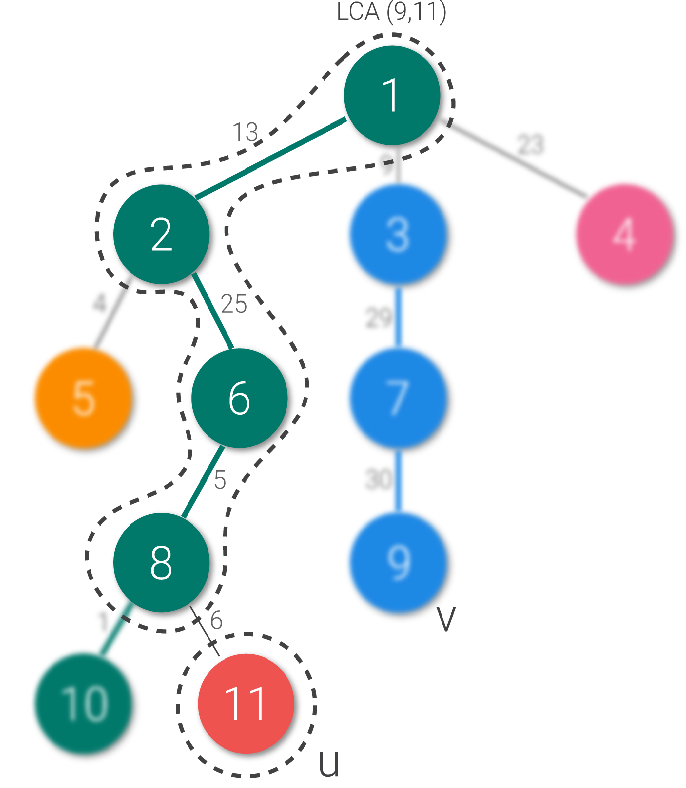
\includegraphics[scale=0.2]{img/heavy-light-decomposition.png}
  \end{center}
  \caption{Heavy Light decomposition of a Tree}
\end{figure}


\section{Basic Algorithms on Graphs}


\subsection{List of algorithms}

\begin{itemize}
  \item Depth First Search
  \item Breadth First Search
  \item Shortest Path - Dijkstra's
  \item Shortest Path - Bellman Ford
  \item Shortest Path - Floyd Warshall
  \item Connected Components
  \item Topological Sort
  \item Prim's Maximum Spanning Tree

\end{itemize}


\subsection{Code}

\lstinputlisting[basicstyle=Large,style=cpp]{code/Graphs.hpp}

\end{document}
